%% beamer/knitr slides 
%% for Statistical Modeling and Data Visualization course @ UMass
%% Nicholas Reich: nick [at] schoolph.umass.edu


\documentclass[table]{beamer}\usepackage[]{graphicx}\usepackage[]{color}
% maxwidth is the original width if it is less than linewidth
% otherwise use linewidth (to make sure the graphics do not exceed the margin)
\makeatletter
\def\maxwidth{ %
  \ifdim\Gin@nat@width>\linewidth
    \linewidth
  \else
    \Gin@nat@width
  \fi
}
\makeatother

\definecolor{fgcolor}{rgb}{0.345, 0.345, 0.345}
\newcommand{\hlnum}[1]{\textcolor[rgb]{0.686,0.059,0.569}{#1}}%
\newcommand{\hlstr}[1]{\textcolor[rgb]{0.192,0.494,0.8}{#1}}%
\newcommand{\hlcom}[1]{\textcolor[rgb]{0.678,0.584,0.686}{\textit{#1}}}%
\newcommand{\hlopt}[1]{\textcolor[rgb]{0,0,0}{#1}}%
\newcommand{\hlstd}[1]{\textcolor[rgb]{0.345,0.345,0.345}{#1}}%
\newcommand{\hlkwa}[1]{\textcolor[rgb]{0.161,0.373,0.58}{\textbf{#1}}}%
\newcommand{\hlkwb}[1]{\textcolor[rgb]{0.69,0.353,0.396}{#1}}%
\newcommand{\hlkwc}[1]{\textcolor[rgb]{0.333,0.667,0.333}{#1}}%
\newcommand{\hlkwd}[1]{\textcolor[rgb]{0.737,0.353,0.396}{\textbf{#1}}}%
\let\hlipl\hlkwb

\usepackage{framed}
\makeatletter
\newenvironment{kframe}{%
 \def\at@end@of@kframe{}%
 \ifinner\ifhmode%
  \def\at@end@of@kframe{\end{minipage}}%
  \begin{minipage}{\columnwidth}%
 \fi\fi%
 \def\FrameCommand##1{\hskip\@totalleftmargin \hskip-\fboxsep
 \colorbox{shadecolor}{##1}\hskip-\fboxsep
     % There is no \\@totalrightmargin, so:
     \hskip-\linewidth \hskip-\@totalleftmargin \hskip\columnwidth}%
 \MakeFramed {\advance\hsize-\width
   \@totalleftmargin\z@ \linewidth\hsize
   \@setminipage}}%
 {\par\unskip\endMakeFramed%
 \at@end@of@kframe}
\makeatother

\definecolor{shadecolor}{rgb}{.97, .97, .97}
\definecolor{messagecolor}{rgb}{0, 0, 0}
\definecolor{warningcolor}{rgb}{1, 0, 1}
\definecolor{errorcolor}{rgb}{1, 0, 0}
\newenvironment{knitrout}{}{} % an empty environment to be redefined in TeX

\usepackage{alltt}


%       ************************************************
%       **        LaTeX preamble to be used with all 
%	**        statsTeachR labs/handouts.
%
%	Author: Nicholas G Reich
%	Last modified: 14 January 2014
%	************************************************

% \documentclass[table]{beamer}

%	Set theme (a nice plain one)
\usetheme{Malmoe}

%	Use named colors, set main color of theme
%		to match Web site color:
\definecolor{MainColor}{RGB}{10, 74, 109}
\colorlet{MainColorMedium}{MainColor!50}
\colorlet{MainColorLight}{MainColor!20}
\usecolortheme[named=MainColor]{structure} 

%	For tables
%[dvipsnames] [table]
\usepackage{xcolor}

%% calling tabu.sty, assuming a particular directory structure
\usepackage{../../slide-includes/tabu}	% Even fancier than tabulary
\usepackage{multirow}

%	Just for the degree symbol
\usepackage{textcomp}

%	Get rid of footline (page, author, etc. on each slide)
\setbeamertemplate{footline}{}
%	Get rid of navigation buttons
\setbeamertemplate{navigation symbols}{}

%	Make footnotes not ugly
\usepackage{hanging}
\setbeamertemplate{footnote}{\raggedright\hangpara{1em}{1}\makebox[1em][l]{\insertfootnotemark}\footnotesize\insertfootnotetext\par}

%	Text style for code snippets inline in text:
\newcommand{\codeInline}[1]{\texttt{#1}}

%	Text style for emphasis stronger than \emph:
%		(Note, this doesn't toggle the way \emph does.
%			(Note, this can be done, didn't seem worth the trouble.))
\newcommand{\strong}[1]{{\bfseries{#1}}}


%        ******	Define title page	**********************
\setbeamertemplate{title page}{
	{\color{MainColor}
	% There must be a better way than this -vspace at
	%	 the top and bottom of the page to reduce the 
	%	 bottom margin, but I can't find one that works.
	\vspace{-6em}

% 	% Go to a lot of trouble to get the title in a
% 	%	nice box, since customizing a beamer block
% 	%	does not entirely work here (I don't know why)
	\newlength{\titleBoxWidth}
	\setlength{\titleBoxWidth}{\textwidth}
	\addtolength{\titleBoxWidth}{-2.0em}
	\setlength{\fboxsep}{1.0em}
	\setlength{\fboxrule}{0pt}
	\fcolorbox{MainColor!25}{MainColor!25}{
		\parbox{\titleBoxWidth}{
			\raggedright
			\LARGE\textbf{\inserttitle}
		}	% end parbox
	}	% end fcolorbox

	\vfill
	\small{Author: \insertauthor}
	\vspace{\baselineskip}

	\small{\Course}

	\small{\Instructor}
	\vspace{\baselineskip}

	%\small{\emph{This material is part of the \strong{statsTeachR} project}}

	\vspace{0.33\baselineskip}\scriptsize{\emph{\LicenseText}}


		\vspace{-15em}

	}	% end color
	\clearpage
}	% end define title page

%	The following variables are assumed by the standard preamble:
%	Global variable containing module name:
\title{Ethics in Data Science}
%	Global variable containing module shortname:
%		(Currently unused, may be used in future.)
\newcommand{\ModuleShortname}{introRegression}
%	Global variable containing author name:
\author{Nicholas G Reich}
%	Global variable containing text of license terms:
\newcommand{\LicenseText}{Made available under the Creative Commons Attribution-ShareAlike 3.0 Unported License: http://creativecommons.org/licenses/by-sa/3.0/deed.en\textunderscore US }
%	Instructor: optional, can leave blank.
%		Recommended format: {Instructor: Jane Doe}
\newcommand{\Instructor}{}
%	Course: optional, can leave blank.
%		Recommended format: {Course: Biostatistics 101}
\newcommand{\Course}{}


\input{../../slide-includes/shortcuts}

\hypersetup{colorlinks,linkcolor=,urlcolor=MainColor}


%	******	Document body begins here	**********************
\IfFileExists{upquote.sty}{\usepackage{upquote}}{}
\begin{document}

%	Title page
\begin{frame}[plain]
	\titlepage
\end{frame}

%	******	Everything through the above line must be placed at
%		the top of any TeX file using the statsTeachR standard
%		beamer preamble. 





%%%%%%%%%%%%%%%%%%%%%%%%%%%%%%%%%%%%%%%%%%

\begin{frame}[fragile]{Research Ethics\footnote{\href{https://xkcd.com/1390/}{https://xkcd.com/1390/}}}

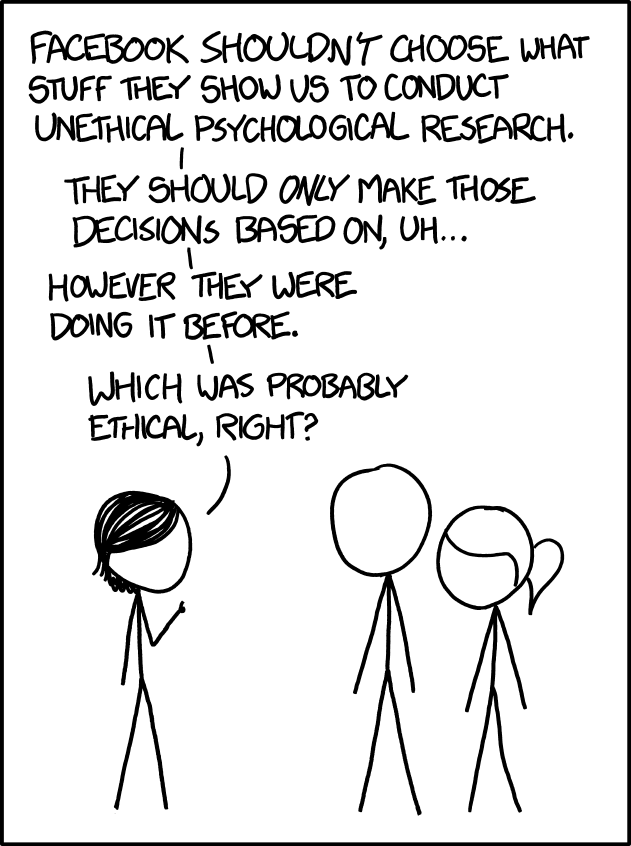
\includegraphics[width=.5\textwidth]{figure-static/research_ethics_2x}

\end{frame}


%%%%%%%%%%%%%%%%%%%%%%%%%%%%%%%%%%%%%%%%%%

\begin{frame}[fragile]{Professional ethics require vigilance, common sense}

\begin{block}{Important to have an open, honest orientation}

\bi

\item Work to be conscious of your and others' biases.
\item Be willing to stand up for what you believe is right.
\item Ask for help when you need it or if you feel unsure.
\item Admit mistakes when you make them.
\item Be open to learn.
\item Create open, transparent, tested workflows.

\ei

\end{block}

\end{frame}

%%%%%%%%%%%%%%%%%%%%%%%%%%%%%%%%%%%%%%%%%%

\begin{frame}[fragile]{Responsibility to stakeholders\footnote{Adapted from {\em Modern Data Science with R}}}

\begin{block}{Know and understand your obligations}

\bi

  \item {\bf Are you legally bound to your employer or client?} What terms and conditions apply?
  \item {\bf Do you have a responsibility to the general public or people whose data you have at your fingertips?} Should you keep datasets on your laptop? etc...
  \item {\bf Are there legal responsibilities that you need to be aware of?} Sometimes, there are legal terms around data sharing and/or confidentiality.
  \item {\bf Are there responsibilities, binding or not, that you have to your professional community?} Make your data and code public, to the extent possible.

\ei

\end{block}

\end{frame}

%%%%%%%%%%%%%%%%%%%%%%%%%%%%%%%%%%%%%%%%%%

\begin{frame}[fragile]{Present results with humility}

\begin{block}{Overconfidence is a common error when interpreting data/models}

\bi
  \item Scrutinize your results from every angle. What would a critic say?
  \item Use language like ``the models says...'' to reinforce that outputs come from a model with assumptions.
  \item Present all evidence honestly, including that which doesn't totally fit the storyline, especially if the story fits your pre-conceived notion. Why are outliers outlying?

\ei

\end{block}

\end{frame}


%%%%%%%%%%%%%%%%%%%%%%%%%%%%%%%%%%%%%%%%%%

\begin{frame}[fragile]{Conflicts of interest (COI)}

\begin{block}{COIs arise frequently and naturally}

\bi
  \item You have a responsibility to identify COIs. e.g. 
  
  \begin{quotation}
    \noindent \small ... I have been paid for my work by Company X.
  \end{quotation}
  
  \begin{quotation}
    \noindent \small ... I have collaborated with colleague Y on a large group project in the last two years. I do not feel that this precludes me from providing an unbiased review of the manuscript.
  \end{quotation}
  
  \item They can become an issue if not identified early.
  \item Often, different fields will have policies and standards in places to ensure reporting and compliance. 
  
\ei

\end{block}

\end{frame}


%%%%%%%%%%%%%%%%%%%%%%%%%%%%%%%%%%%%%%%%%%

\begin{frame}[fragile]{Acknowledge mistakes}

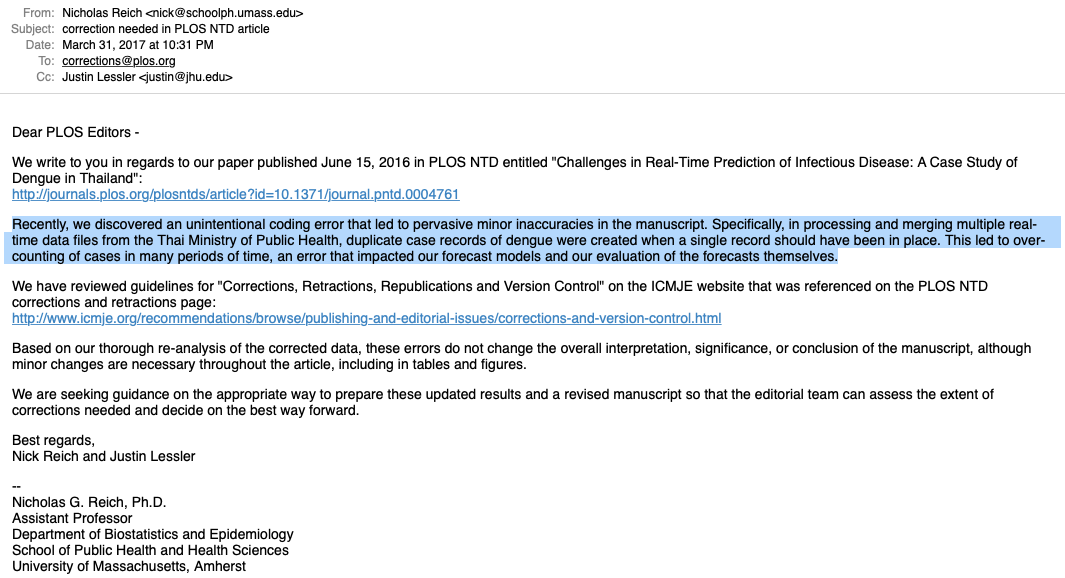
\includegraphics[width=\textwidth]{figure-static/email-to-plos}

\end{frame}

%%%%%%%%%%%%%%%%%%%%%%%%%%%%%%%%%%%%%%%%%%

\begin{frame}[fragile]{Ethical principles for data science\footnote{Adapted from {\em Modern Data Science with R}}}

\begin{block}{Summary of key points}

\bi

  \item Do your work well by your own standards and by the standards of your profession.
  \item Recognize the parties to whom you have a special professional obligation.
  \item Report results and methods honestly 
  \teim Respect your responsibility to identify and report flaws and shortcomings in your work.
  \item Acknowledge possible conflicts of interest at appropriate times.

\ei

\end{block}

\end{frame}



\end{document}
